\documentclass[a4paper,12pt]{memoir} % Font and paper size

%%%%%%%%%%%%%%%%%%%%%%%%%%%%%%%%%%%%%%%%%
% Wenneker Resume/CV
% Structure Specification File
% Version 1.1 (19/6/2016)
%
% This file has been downloaded from:
% http://www.LaTeXTemplates.com
%
% Original author:
% Frits Wenneker (http://www.howtotex.com) with extensive modifications by 
% Vel (vel@latextemplates.com)
%
% License:
% CC BY-NC-SA 3.0 (http://creativecommons.org/licenses/by-nc-sa/3.0/)
%
%%%%%%%%%%%%%%%%%%%%%%%%%%%%%%%%%%%%%%%%%

%----------------------------------------------------------------------------------------
%	PACKAGES AND OTHER DOCUMENT CONFIGURATIONS
%----------------------------------------------------------------------------------------

\usepackage{XCharter} % Use the Bitstream Charter font
\usepackage[utf8]{inputenc} % Required for inputting international characters
\usepackage[T1]{fontenc} % Output font encoding for international characters

\usepackage[top=1cm,left=1cm,right=1cm,bottom=1cm]{geometry} % Modify margins

\usepackage{graphicx} % Required for figures

\usepackage{flowfram} % Required for the multi-column layout

\usepackage{url} % URLs

\usepackage[usenames,dvipsnames]{xcolor} % Required for custom colours

\usepackage{tikz} % Required for the horizontal rule

\usepackage{enumitem} % Required for modifying lists
\setlist{noitemsep,nolistsep} % Remove spacing within and around lists

\setlength{\columnsep}{\baselineskip} % Set the spacing between columns

% Define the left frame (sidebar)
\newflowframe{0.2\textwidth}{\textheight}{0pt}{0pt}[left]
\newlength{\LeftMainSep}
\setlength{\LeftMainSep}{0.2\textwidth}
\addtolength{\LeftMainSep}{1\columnsep}
 
% Small static frame for the vertical line
\newstaticframe{1.5pt}{\textheight}{\LeftMainSep}{0pt}
 
% Content of the static frame with the vertical line
\begin{staticcontents}{1}
\hfill
\tikz{\draw[loosely dotted,color=RoyalBlue,line width=1.5pt,yshift=0](0,0) -- (0,\textheight);}
\hfill\mbox{}
\end{staticcontents}
 
% Define the right frame (main body)
\addtolength{\LeftMainSep}{1.5pt}
\addtolength{\LeftMainSep}{1\columnsep}
\newflowframe{0.7\textwidth}{\textheight}{\LeftMainSep}{0pt}[main01]

\pagestyle{empty} % Disable all page numbering

\setlength{\parindent}{0pt} % Stop paragraph indentation

%----------------------------------------------------------------------------------------
%	NEW COMMANDS
%----------------------------------------------------------------------------------------

\newcommand{\userinformation}[1]{\renewcommand{\userinformation}{#1}} % Define a new command for the CV user's information that goes into the left column

\newcommand{\cvheading}[1]{{\Huge\bfseries\color{RoyalBlue} #1} \par\vspace{.6\baselineskip}} % New command for the CV heading
\newcommand{\cvsubheading}[1]{{\Large\bfseries #1} \bigbreak} % New command for the CV subheading

\newcommand{\Sep}{\vspace{1em}} % New command for the spacing between headings
\newcommand{\SmallSep}{\vspace{0.5em}} % New command for the spacing within headings

\newcommand{\aboutme}[2]{ % New command for the about me section
\textbf{\color{RoyalBlue} #1}~~#2\par\Sep
}
	
\newcommand{\CVSection}[1]{ % New command for the headings within sections
{\Large\textbf{#1}}\par
\SmallSep % Used for spacing
}

\newcommand{\CVItem}[2]{ % New command for the item descriptions
\textbf{\color{RoyalBlue} #1}\par
#2
\SmallSep % Used for spacing
}

\newcommand{\bluebullet}{\textcolor{RoyalBlue}{$\circ$}~~} % New command for the blue bullets
 % Include the file specifying document layout and packages

%----------------------------------------------------------------------------------------
%	NOMBRE Y CONTACTO
%----------------------------------------------------------------------------------------

\userinformation{ % Set the content that goes into the sidebar of each page
\begin{flushright}
% Comment out this figure block if you don't want a photo
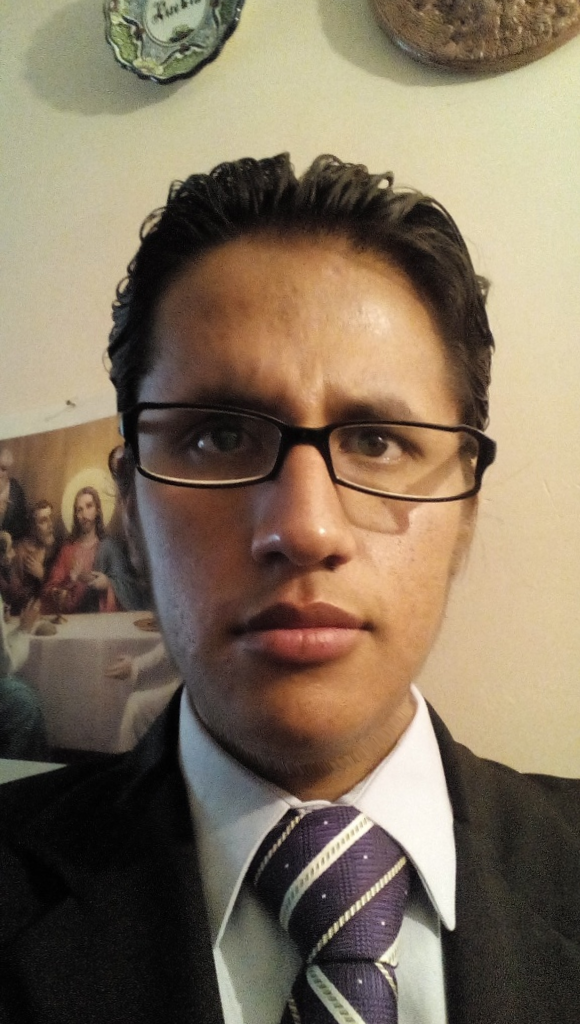
\includegraphics[width=0.6\columnwidth]{yap.jpeg}\\[\baselineskip] % Your photo
\small % Smaller font size
Julio Cesar\\ Enciso Alva \\ % Your name
\url{enciso.alva.jc@gmail.com} \\ % Your email address
%\url{www.johnsmith.com} \\ % Your URL
(044) 771 158 55 65 \\ % Your phone number
\Sep % Some whitespace
\textbf{Dirección} \\
Cedro 209,\\ Fracc. Tulipanes \\ % Address 1
Mral. de la Reforma, Hidalgo \\ % Address 2
CP 42185 \\ % Address 3
\vfill % Whitespace under this block to push it up under the photo
\end{flushright}
}

%----------------------------------------------------------------------------------------

\begin{document}

\userinformation % Print your information in the left column

\framebreak % End of the first column

%----------------------------------------------------------------------------------------
%	ENCABEZADO
%----------------------------------------------------------------------------------------

\cvheading{Julio Cesar Enciso Alva} % Large heading - your name

\cvsubheading{Lic. Matemáticas Aplicadas} % Subheading - your occupation/specialization

%----------------------------------------------------------------------------------------
%	EDUCATION
%----------------------------------------------------------------------------------------

\CVSection{Educación}

%------------------------------------------------

\CVItem{2012 - 2017, Universidad Autónoma del Estado de Hidalgo}
{Licenciatura en Matemáticas Aplicadas, subespecialidad en Biología}

%------------------------------------------------

\CVItem{2009 - 2012, Preparatoria 3 (UAEH)}{Bachillerato General}

\Sep % Extra whitespace after the end of a major section

%----------------------------------------------------------------------------------------
%	EXPERIENCIA
%----------------------------------------------------------------------------------------

\CVSection{Experiencia}

\CVItem{Enero - Julio 2017, \textit{Programa 'Cuenta Conmigo'}, UAEH}
{Apoyo extraescolar para estudiantes de primarias y secundarias públicas en la ciudad de Pachuca
y sus alrededores.}

%------------------------------------------------

\CVItem{Agosto - Diciembre 2016, \textit{Olimpiada de Matemáticas}, Preparatoria 3}
{Asesorías para un grupo de estudiantes
como preparación para la Olimpiada Hidalguense de Matemáticas 2017, obteniéndose
dos primeros lugares y un segundo lugar.}

%------------------------------------------------

%\CVItem{Agosto 2014 - Junio 2015, \textit{Asistente educativo}, CIFUNHI A.C.}
%{Apoyo educativo para ni\~nos (10-12 a\~nos) con discapacidad visual.}

\Sep % Extra whitespace after the end of a major section

%----------------------------------------------------------------------------------------
%	COMMUNICATION SKILLS
%----------------------------------------------------------------------------------------

\CVSection{Eventos destacados}

\CVItem{Julio 2017, \textit{Neuroscience Short Course}, UAEH}
{Expositor en el módulo '\textit{Mathematics and Neuroscience}' sobre análisis de señales
electrofisiológicas. Evento interdisciplinario entre las áreas académicas de Gerontología,
Psicología y Matemáticas de la UAEH.}

\CVItem{Octubre 2016, \textit{Congreso Nacional de la SMM}, Aguascalientes}
{Presentación de resultados de tesis en el 49 Congreso Nacional de la 
Sociedad Matemática Mexicana, bajo el título 
'\textit{Aplicación de pruebas de estacionariedad débil en
series electrofisiológicas}'.}

\CVItem{Diciembre 2015, \textit{VII Coloquio de Matemática Educativa}, UAEH}
{Asistente y voluntario. Evento dirigido a profesores de materias relacionadas a 
matemáticas en nivel básico, medio superior y superior, organizado por el Centro de
Investigación en Matemáticas de la UAEH.}

\Sep % Extra whitespace after the end of a major section

%----------------------------------------------------------------------------------------
%	COMPETENCIAS
%----------------------------------------------------------------------------------------

\CVSection{Competencias}

\CVItem{Computación}{
\begin{itemize}
\item[\bluebullet] Fluidez en Windows y Linux
\item[\bluebullet] Dominio de Microsoft Office, Libre Office, LaTeX
\item[\bluebullet] Manejo de Dropbox, Google Drive, One Note
\item[\bluebullet] Apoyo didáctico con Geogebra, Cabri, PSeInt
\item[\bluebullet] Lenguajes de programación: C/C++, python, R, Matlab/Octave
\end{itemize}}
%{\begin{tabular}{p{0.2\textwidth} p{0.2\textwidth} p{0.2\textwidth}}
%\bluebullet  &  \bluebullet Shell & \bluebullet Python\\
%\bluebullet C++ &  \bluebullet PHP & \bluebullet Matlab\\
%\end{tabular}}

%------------------------------------------------

\CVItem{Idiomas}{
\begin{itemize}
\item[\bluebullet] Inglés (B2, TOEFL)
\item[\bluebullet] Alemán (B1, Zertifikat in Deutsch)
\end{itemize}}
%\CVItem{Computer Software}
%{\begin{tabular}{p{0.2\textwidth} p{0.2\textwidth} p{0.2\textwidth}}
% \bluebullet MySQL &  \bluebullet iOS & \bluebullet Android\\
%\end{tabular}}

%------------------------------------------------

\Sep % Extra whitespace after the end of a major section

%----------------------------------------------------------------------------------------
%	NEW PAGE DELIMITER
%	Place this block wherever you would like the content of your CV to go onto the next page
%----------------------------------------------------------------------------------------

%\clearpage % Start a new page
%
%\userinformation % Print your information in the left column
%
%\framebreak % End of the first column

%----------------------------------------------------------------------------------------
%	INTERESTS
%----------------------------------------------------------------------------------------

%\CVSection{Intereses}
%
%\CVItem{Profesional}{Series de tiempo, Procesamiento de se\~nales, Electrofisiología 
%cuantitativa, Sistemas dinámicos, Métodos numéricos, Didáctica de las matemáticas 
%(especialmente propiedades locales)}
%
%%------------------------------------------------
%
%\CVItem{Personal}{Ajedrez, juegos de mesa, videojuegos, dise\~no gráfico, jardineróa}
%
%\Sep % Extra whitespace after the end of a major section

%----------------------------------------------------------------------------------------

\end{document}